\documentclass{article}
\usepackage{amsmath} % need to be on top for eps files
\usepackage{caption}
\usepackage{subcaption}
\usepackage{graphicx}
\graphicspath{ {latex/Images/} }
\usepackage{epstopdf} 


%% sidebyside images


%%%%%%%%%%%%%%%%%%%%%%%%%%%%%%%%%%%%%%%%%%%%%%%%%% Create listings (Matlab)
% % Create a matlab listing
\usepackage{listings}
\usepackage{color} %red, green, blue, yellow, cyan, magenta, black, white
\definecolor{mygreen}{RGB}{28,172,0} % color values Red, Green, Blue
\definecolor{mylilas}{RGB}{170,55,241}

\usepackage[utf8]{inputenc}
\usepackage{geometry}
 \geometry{
 a4paper,
 total={175mm,265mm},
 left=15mm,
 top=15mm,
 }
\usepackage{amsmath}%To be able to use split in equation


%%%% Include eps files:
\usepackage{amsmath} % need to be on top for eps files
\usepackage{graphicx}
%set the relative location for eps files
\graphicspath{ {/images/} }
\usepackage{listings}
\usepackage{cleveref} %cleverref needs to stand below amsmath package.
\usepackage{graphicx}
\usepackage{float}
%\usepackage{hyperref}
\usepackage{url} %To be able to use url in references
\usepackage{graphicx}
\usepackage{tabularx} % in the preamble
\usepackage{wrapfig}

%\usepackage{algorithm}
%\usepackage{algorithmic}


% To get side by side pictures:{
\usepackage{caption}
\usepackage{subcaption}
\usepackage{graphicx}




%%%%%%%%%%%%%%%%%%%%%%%%%%%%%%%%%%%%%%%%%%%%%%%%%% Create listings (Python)
% set code color pattern (for python)
% Default fixed font does not support bold face
\DeclareFixedFont{\ttb}{T1}{txtt}{bx}{n}{12} % for bold
\DeclareFixedFont{\ttm}{T1}{txtt}{m}{n}{12}  % for normal

% Custom colors
\usepackage{color}
\definecolor{deepblue}{rgb}{0,0,0.5}
\definecolor{deepred}{rgb}{0.6,0,0}
\definecolor{deepgreen}{rgb}{0,0.5,0}

\usepackage{listings}

% Python style for highlighting
\newcommand\pythonstyle{\lstset{
language=Python,
breaklines=true, % wrap lines
postbreak=\mbox{\textcolor{red}{$\hookrightarrow$}\space}, % wrap lines
basicstyle=\ttm,
otherkeywords={self},             % Add keywords here
keywordstyle=\ttb\color{deepblue},
emph={MyClass,__init__},          % Custom highlighting
emphstyle=\ttb\color{deepred},    % Custom highlighting style
stringstyle=\color{deepgreen},
frame=tb,                         % Any extra options here
showstringspaces=false            % 
}}

% Python environment
\lstnewenvironment{python}[1][]
{
\pythonstyle
\lstset{#1}
}
{}

% Python for external files
\newcommand\pythonexternal[2][]{{
\pythonstyle
\lstinputlisting[#1]{#2}}}

% Python for inline
\newcommand\pythoninline[1]{{\pythonstyle\lstinline!#1!}}


% Include path to images
\graphicspath{{images/}{latex/project3/}}

% Include pdf files in report
\usepackage{pdfpages}


\usepackage{cleveref} %cleverref needs to stand below amsmath package.
\usepackage{appendix}
\crefname{appsec}{Appendix}{Appendices} % refer to appendix as appendix iso as section (use with text in
\title{Example to plot directly into latex}
%\author{Authors:\\a-t-0}


\date{19-10-2019}
\begin{document}
\crefname{lstlisting}{listing}{listings}
\Crefname{lstlisting}{Listing}{Listings}
%%%%%%%%%%Configure matlab listing%%%%%%%%%%%%%%%%%%
% Specify matlab listing style
\lstset{language=Matlab,%
    %basicstyle=\color{red},
    breaklines=true,%
    morekeywords={matlab2tikz},
    keywordstyle=\color{blue},%
    morekeywords=[2]{1}, keywordstyle=[2]{\color{black}},
    identifierstyle=\color{black},%
    stringstyle=\color{mylilas},
    commentstyle=\color{mygreen},%
    showstringspaces=false,%without this there will be a symbol in the places where there is a space
    numbers=left,%
    numberstyle={\tiny \color{black}},% size of the numbers
    numbersep=9pt, % this defines how far the numbers are from the text
    emph=[1]{for,end,break},emphstyle=[1]\color{red}, %some words to emphasise
    %emph=[2]{word1,word2}, emphstyle=[2]{style},    
}


\maketitle
%\setcounter{chapter}{-1}
%\section{Introduction}\label{sec:intro}
% 3 lines max?:) %\newpage
%\section{Genetic Algorithm Performance}\label{sec:1}
To illustrate how the python code exports the figures directly into the report, this second "hw2" is included. Below are the pictures that are created by the code listed in \cref{app:1} and \cref{app:2}.
\begin{figure}[H]
    \centering
    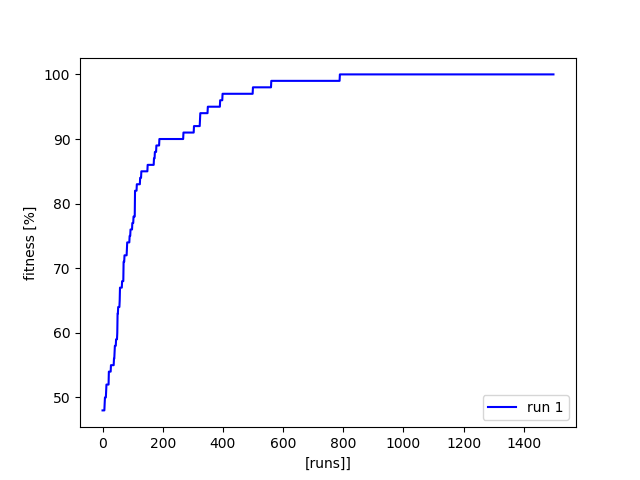
\includegraphics[width=1\textwidth]{Images/4a.png}
    \caption{Performance of some genetic algorithm}
\end{figure}

\begin{figure}[H]
    \centering
    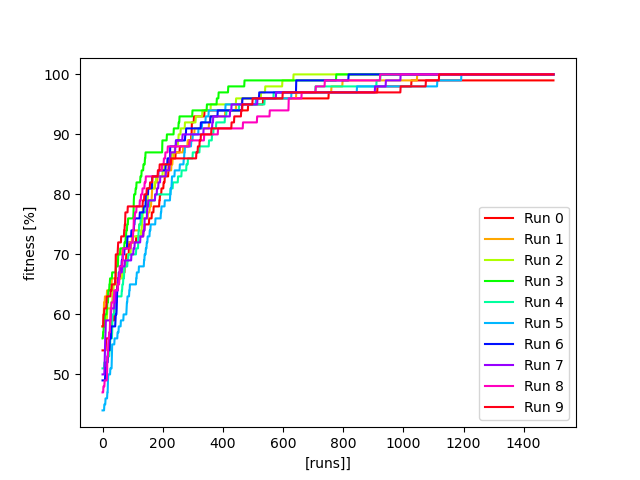
\includegraphics[width=1\textwidth]{Images/4b.png}
    \caption{Performance of some genetic algorithm}
\end{figure} %\newpage
%\input{Chapters/Conclusion.tex} %\newpage
\section{Introduction}\label{sec:intro}
% 3 lines max?:) %\newpage
\section{Genetic Algorithm Performance}\label{sec:1}
To illustrate how the python code exports the figures directly into the report, this second "hw2" is included. Below are the pictures that are created by the code listed in \cref{app:1} and \cref{app:2}.
\begin{figure}[H]
    \centering
    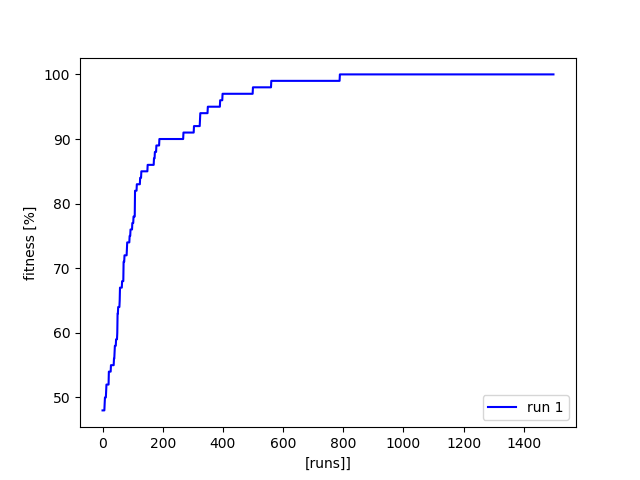
\includegraphics[width=1\textwidth]{Images/4a.png}
    \caption{Performance of some genetic algorithm}
\end{figure}

\begin{figure}[H]
    \centering
    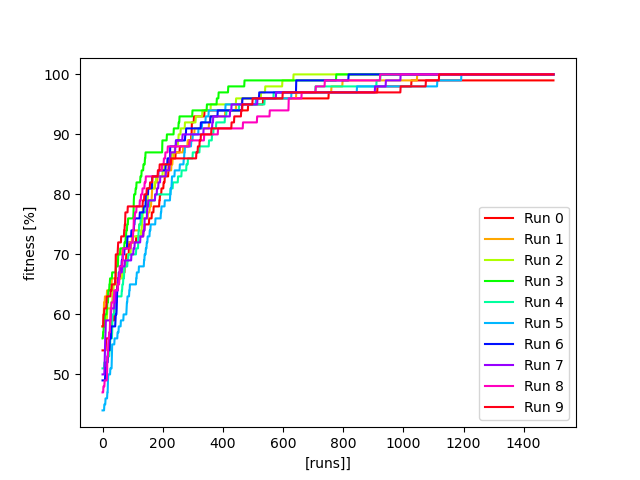
\includegraphics[width=1\textwidth]{Images/4b.png}
    \caption{Performance of some genetic algorithm}
\end{figure} %\newpage















\bibliographystyle{plain} %plain style
\bibliography{references}
\addcontentsline{toc}{chapter}{Bibliography}

\begin{appendices}
\crefalias{section}{appsec}
\newpage
\section{Appendix \_\_main\_\_.py}\label{app:1}
\pythonexternal{latex/project3/../../code/project3/src/__main__.py} \newpage
\section{Appendix Main.py}\label{app:2}
\pythonexternal{latex/project3/../../code/project3/src/Main.py} \newpage
\section*{Appendix python code that exports figures to latex}\label{app:3}
\pythonexternal{latex/project3/../../code/project3/src/Plot_to_tex.py} \newpage
\section*{Appendix python code that compiles the latex report to pdf}\label{app:4}
\pythonexternal{latex/project3/../../code/project3/src/Compile_latex.py} \newpage
\section*{Appendix python code that runs the jupyter notebook(s)}\label{app:5}
\pythonexternal{latex/project3/../../code/project3/src/Run_jupyter_notebooks.py} \newpage
\section*{Appendix Example Jupyter Notebook}\label{app:6}
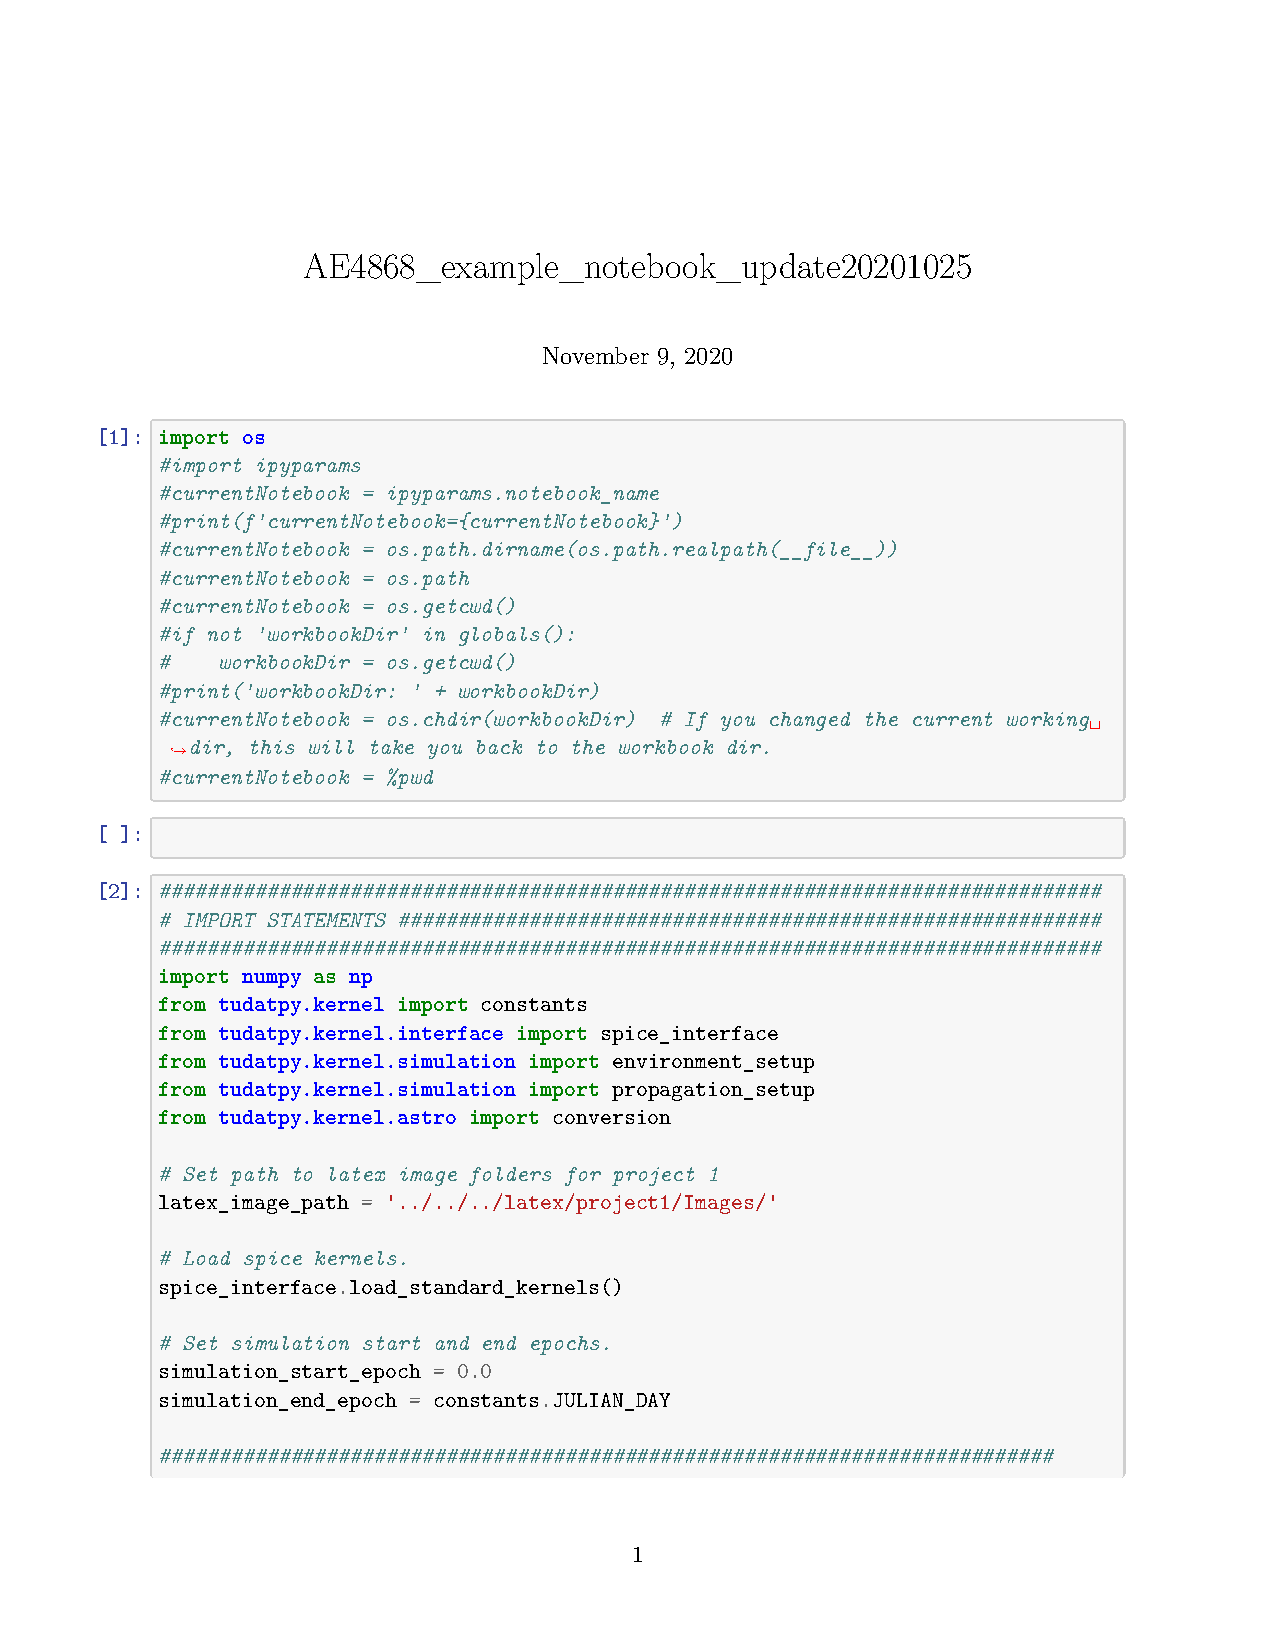
\includepdf[pages=-]{latex/project3/../../code/project3/src/AE4868_example_notebook_update20201025.pdf} \newpage
\end{appendices}

\end{document}
